\documentclass[10pt]{beamer}

\usepackage{graphicx}
\usepackage{ragged2e}
\usepackage[utf8]{inputenc}
\setbeamertemplate{frametitle}[default][center]
\centering

\usepackage{subfigure}
\usepackage[sc]{mathpazo}
\setbeamercovered{dynamic}

%gets rid of bottom navigation bars
\setbeamertemplate{footline}[page number]{}
\setbeamertemplate{navigation symbols}{}


\title{Markov State Models for Simulation Analysis}

\author{Kyle Beauchamp, Robert McGibbon}

\begin{document}

\begin{frame}{MSMBuilder Requirements}
 
\begin{enumerate}
 \item Linux or OSX
 \item Enthough Python Distribution or a Ubuntu VM
 \item MSMBuilder (https://github.com/SimTk/msmbuilder)
 \item CPU with SSE3 support.
 \item GCC 4.2 or later (with OpenMP support)
 \item pymol (optional for visualization)

\end{enumerate} 
 
\end{frame}


\begin{frame}
 \maketitle
\end{frame}

\begin{frame}{Conformational States of Biological Molecules}{Protein Folding}

 
\includegraphics[width=85mm]{Figures/SequenceLogo} 

\large{$\downarrow$}

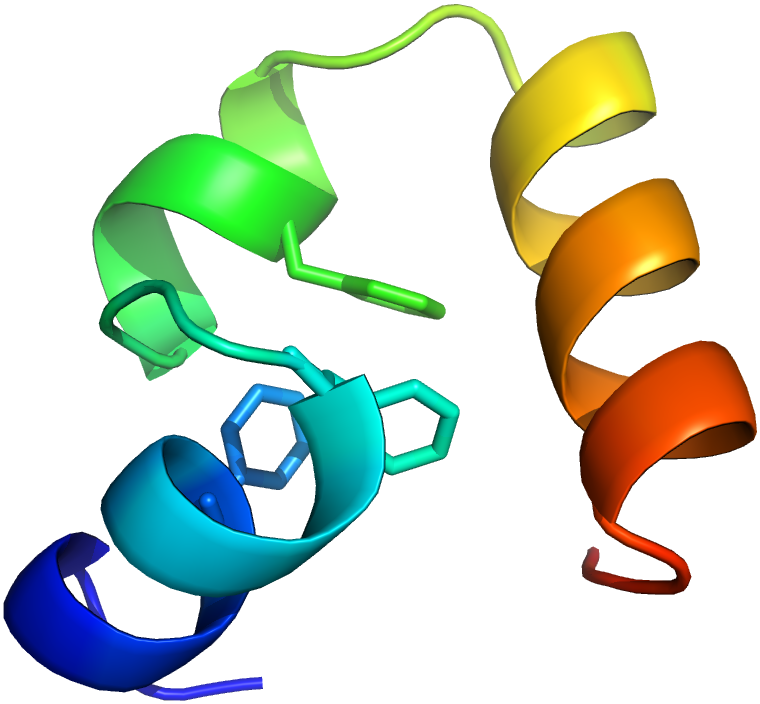
\includegraphics[width=45mm]{Figures/StructureForLogo}

\end{frame}


\begin{frame}{Conformational States of Biological Molecules}{GPCR Dynamics}
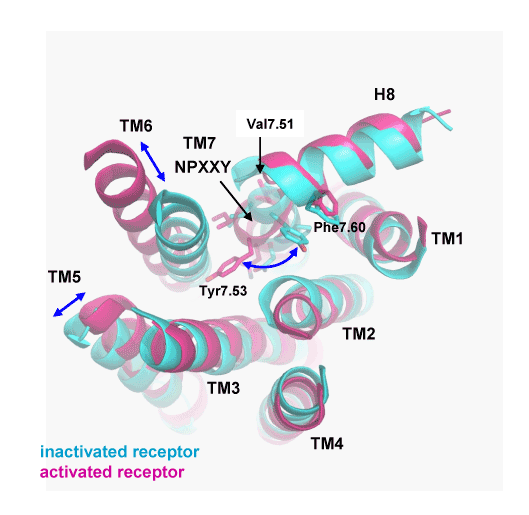
\includegraphics[width=7.0cm]{Figures/GPCR.png}

\tiny
Jean-Francois Deleuze, 2010 

\end{frame}

\begin{frame}{Conformational States of Biological Molecules}{Riboswitches}
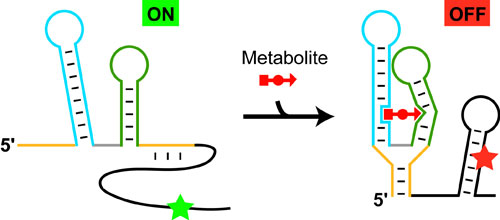
\includegraphics[width=7.0cm]{Figures/Riboswitch.jpg}

\begin{tiny}
Breaker et al
\end{tiny}

\vfill

\begin{center}
 Key Points:
\end{center}


\begin{itemize}
 \item Importance of conformation
 \item Multiple States
 \item Dynamics
\end{itemize}
\end{frame}

\begin{frame}{Molecular Dynamics}
 
Molecular dynamics simulations capture equilibrium and kinetic properties of biomolecules.

\vfill

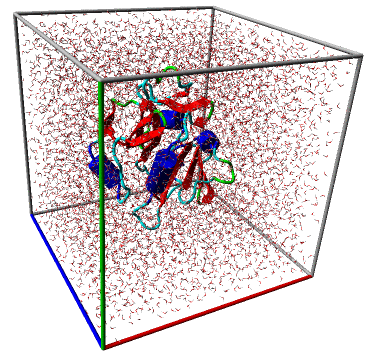
\includegraphics[width=40mm]{Figures/Box}

 
\end{frame}

\begin{frame}{How should we analyze simulation?}
 
 \begin{enumerate}
  \item Direct, quantitative connection to experimental observables
  \item Intuitive explanation (coarse-graining)
  \item Statistically optimal use of limited data
  \item Computationally tractable and easy-to-use
  \item Compatible with both many and few-state behavior
 \end{enumerate}

 \vfill
 
Markov State Models achieve these goals!
 
\end{frame}



\begin{frame}{States and Rates}{Experimentalists view biomolecules through the lens of ``states and rates''}
 
 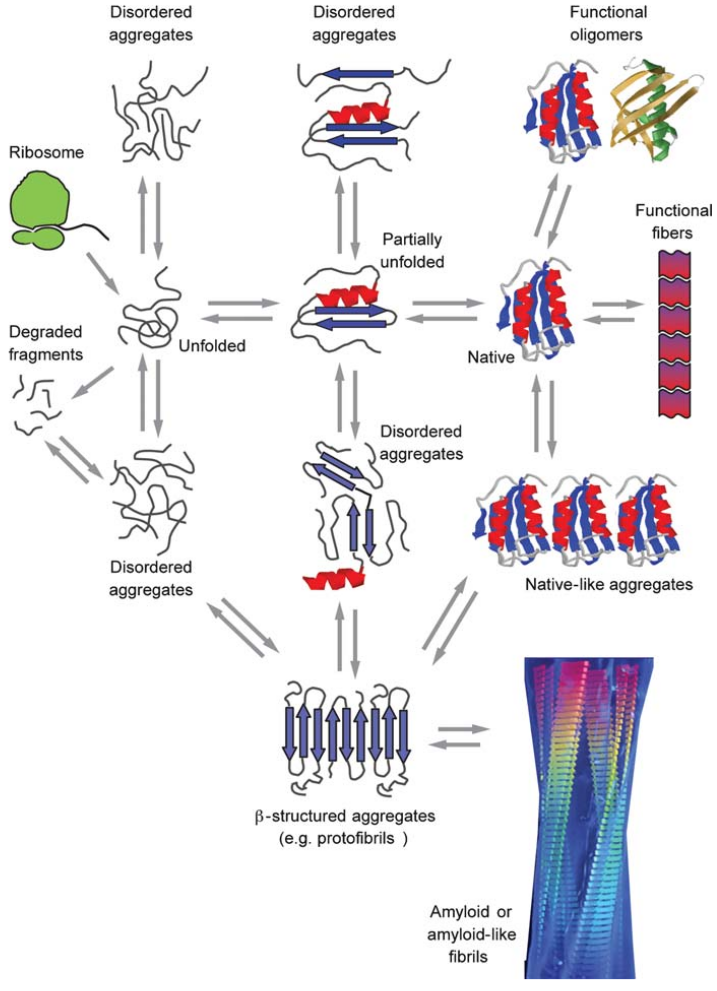
\includegraphics[width=55mm]{Figures/misfolding_dobson2006}
 
  \tiny Dobson, 2006.
 
\end{frame}

\begin{frame}{States and Rates}{Markov State Models provide a ``states and rates'' view on conformational dynamics}
 
 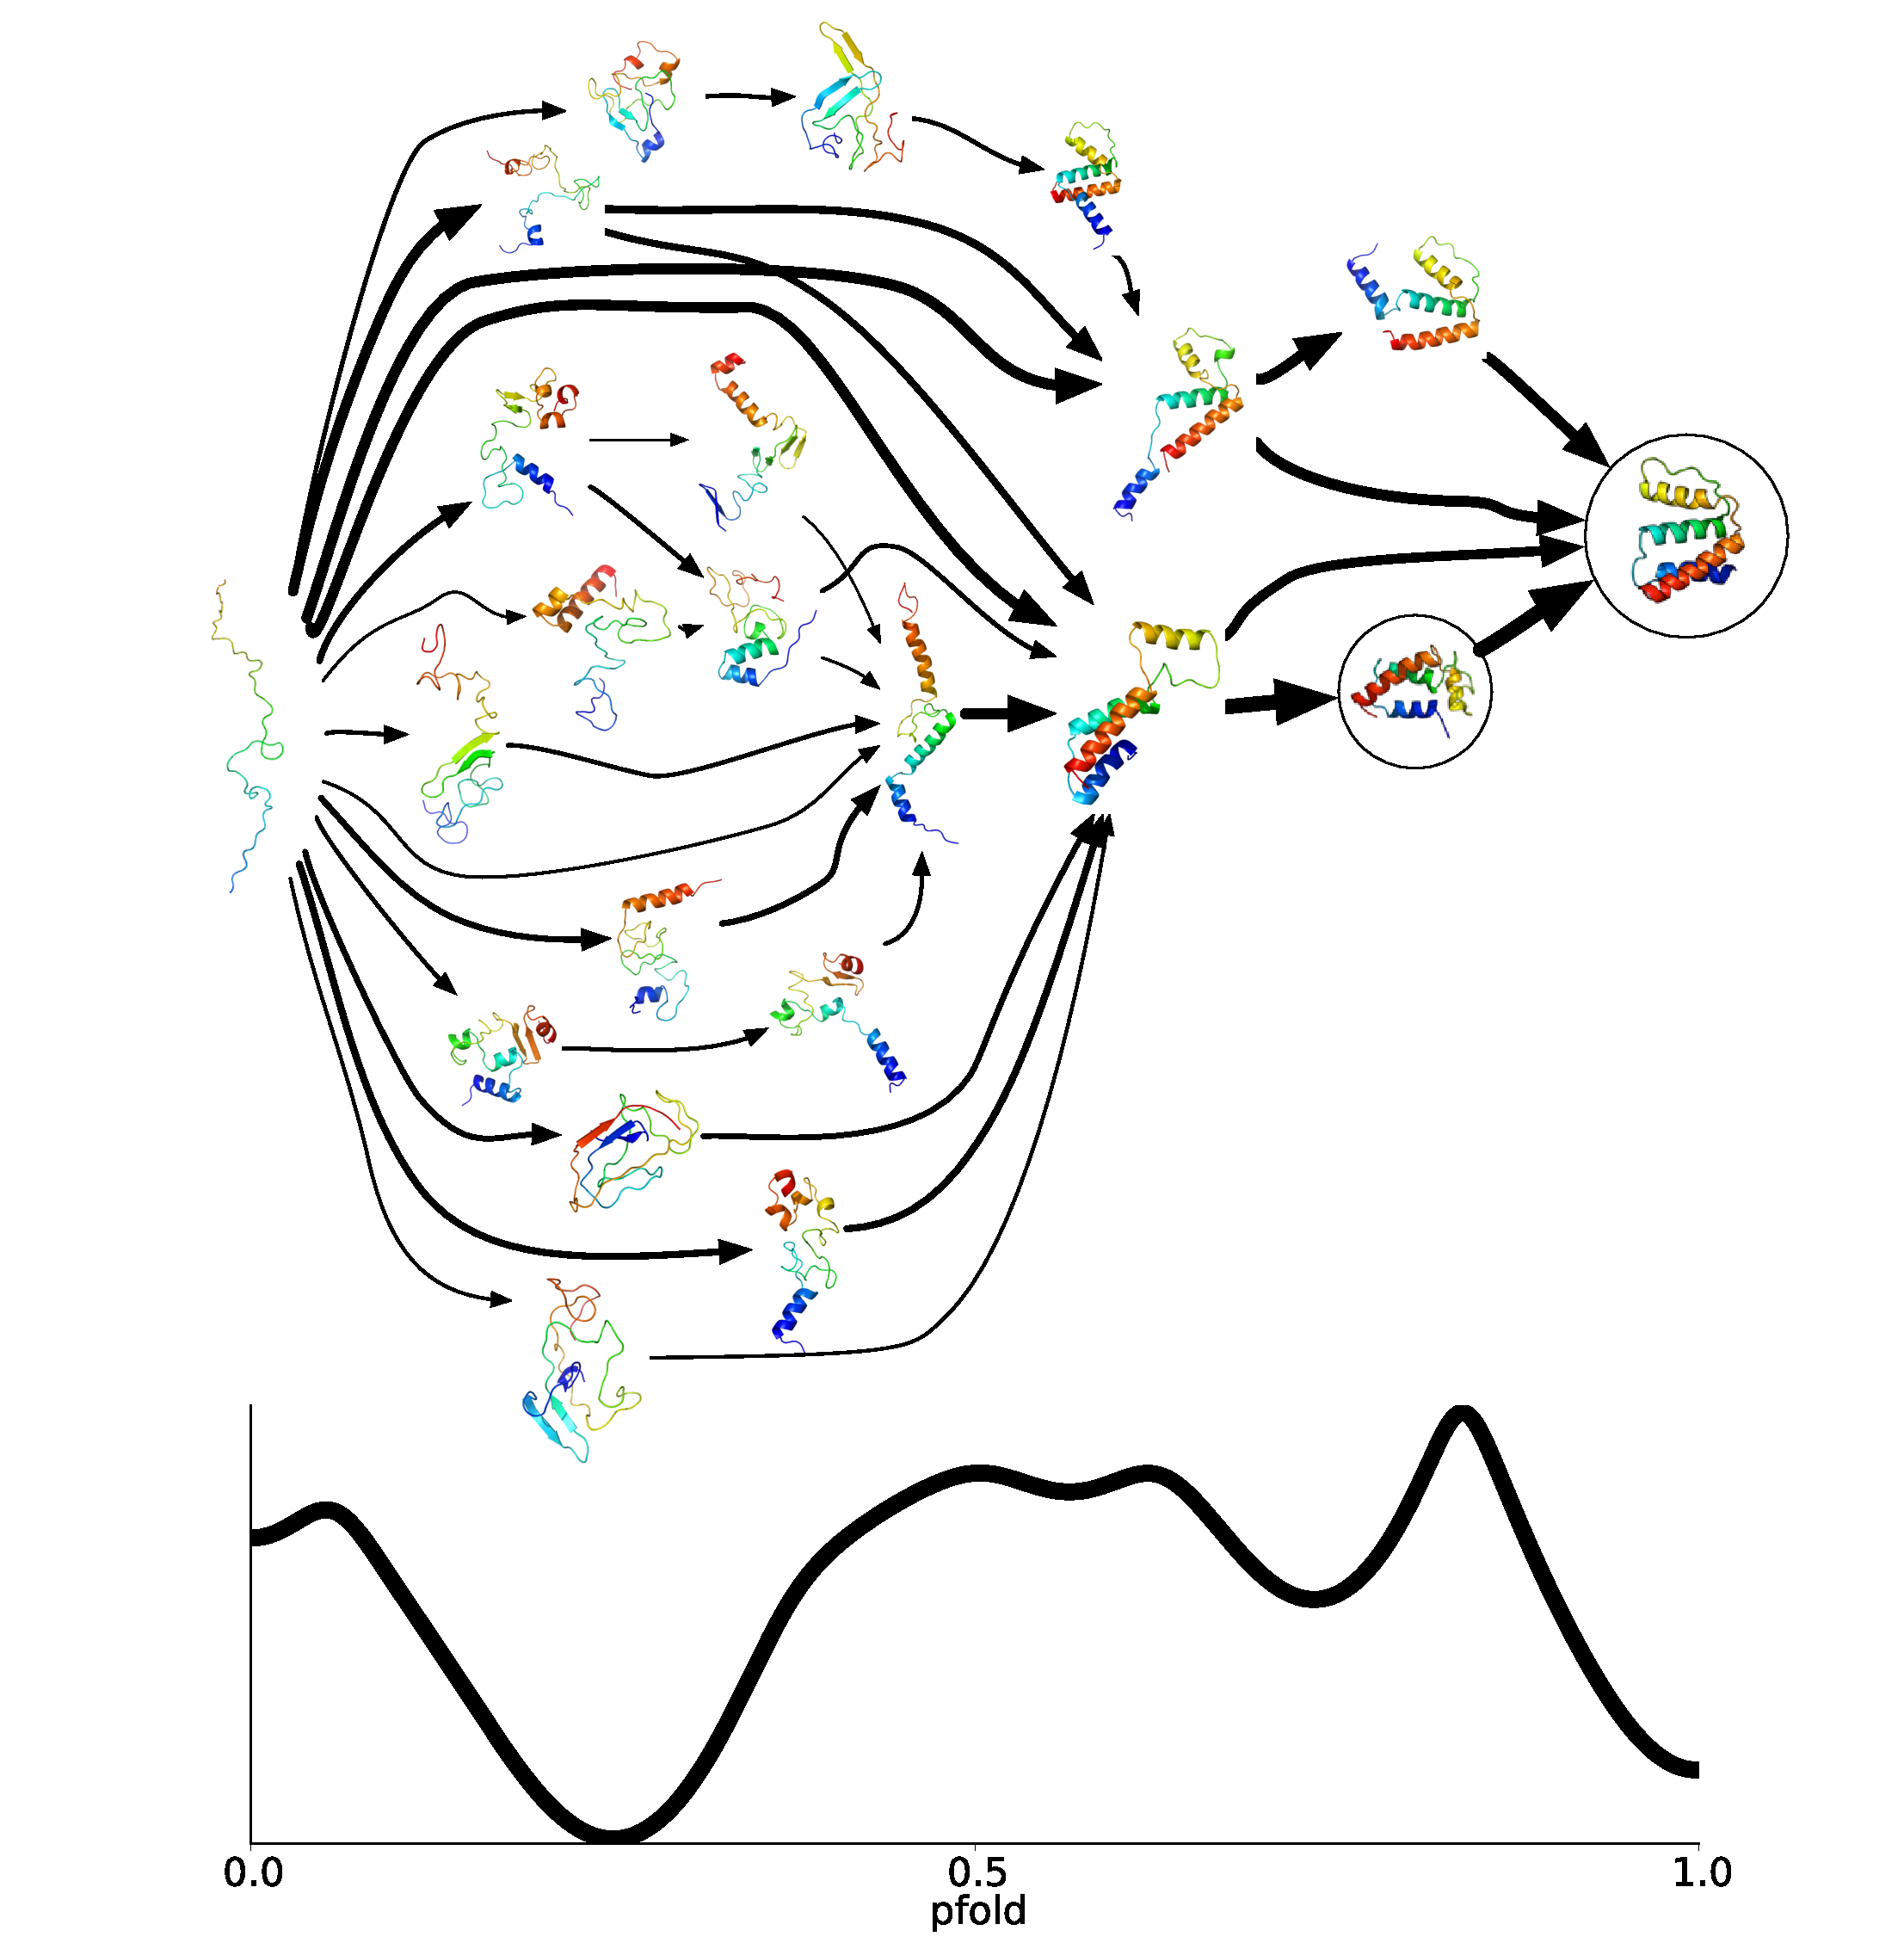
\includegraphics[width=80mm]{Figures/coordinate}
 
  \tiny Voelz et al.
 
\end{frame}

\begin{frame}{Markov State Models in a Nutshell}

\begin{enumerate}
 \item Define states by clustering.
 \item Estimate rates between states.
\end{enumerate}

\end{frame}


\begin{frame}{Markov State Models}

Suppose we have an ensemble of molecular dynamics trajectories: 

\begin{center}
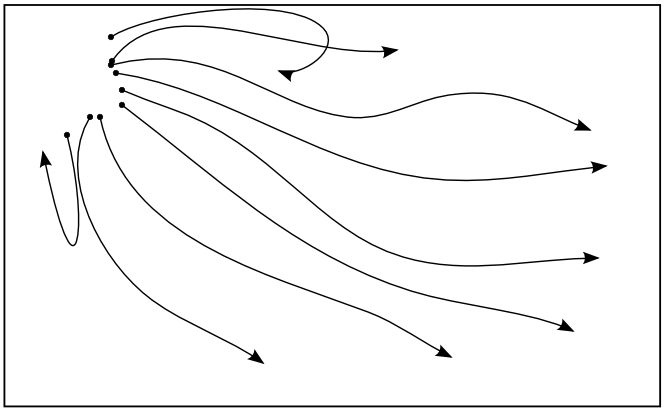
\includegraphics[width=50mm]{Figures/NewPaths2}
\end{center}

\end{frame}

\begin{frame}{Markov State Models}
 
Cluster the conformation space into disjoint states: $\{1,2,3,4,5\}$
\vspace{4mm}
\begin{center}
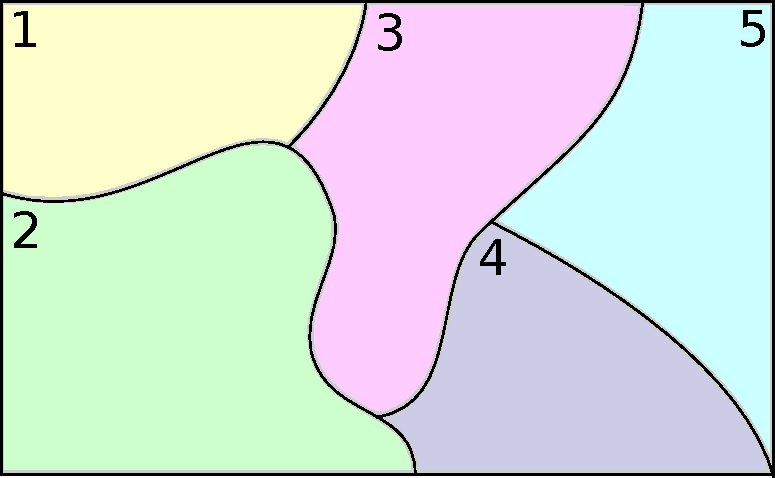
\includegraphics[width=50mm]{Figures/Paths-Clusters}
\end{center}


\end{frame}

\begin{frame}{Markov State Models}
 
Estimate the transition probabilities by counting jumps between states:

\vspace{4mm}
\begin{center}
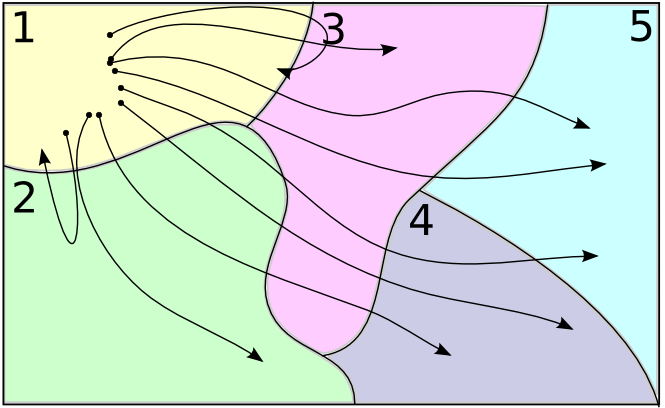
\includegraphics[width=50mm]{Figures/NewPaths3}
\end{center}


\end{frame}

\begin{frame}{Estimating Transition Probabilities}
 
 Suppose we slice our trajectories every $\Delta t$ picoseconds (lagtime) and count the observed transitions:
 
 $$C_{ij} = C_{i \rightarrow j}$$
 
\end{frame}

\begin{frame}{Estimating Transition Probabilities}
 
 To get the transition probabilities, we simply ``normalize'' the counts:
 
 $$T_{ij} = T_{i\rightarrow j}  = \frac{C_{ij}}{\sum_k C_{ik}}$$
 
\end{frame}

\begin{frame}{Dynamics in an MSM}
 
 Suppose that at time zero a protein sits in state $i$.  
 
\vspace{5mm} 

 After lagtime $\Delta t$, jump to another state with probabilities $T_{ij}$.  
 
 \end{frame}
 
 \begin{frame}{Dynamics in an MSM}
 
 Suppose have an ensemble of proteins occupying different states--we describe this by a population vector $\bf{x}(0)$.
 
 $$\bf{x}(t) = T \bf{x}(0)$$
 
\end{frame}

\begin{frame}{Eigenvalues and Eigenvectors}{Equilibrium}
 
 $$T v = \lambda v$$
 
 Setting $\lambda = 1$ gives us the equilibrium populations:
 
 $$T \pi = 1 \pi = \pi$$
 
 At long times, the system approaches equilibrium populations:
 
 $$x(t) \rightarrow \pi$$
 
\end{frame}

\begin{frame}{Eigenvalues and Eigenvectors}{Dynamics}
 
 $$T v = \lambda_i v$$
 
For the remaining eigenvalues, $\lambda_i < 1$.

These eigenvalues correspond to characteristic timescales at which different populations approach equilibrium.

$$ \tau_i = -\frac{\Delta t}{\log \lambda_i}$$
 
 
\end{frame}

\begin{frame}{Eigenvalues and Eigenvectors}{Projection}
 
Suppose we have an experiment that monitors a single variable $y(t)$.  

$$y(t) = \sum_i c_i \exp (-\frac{t}{t_i})   <\mathbf{v_i}, \mathbf{x}(0)> $$
 
  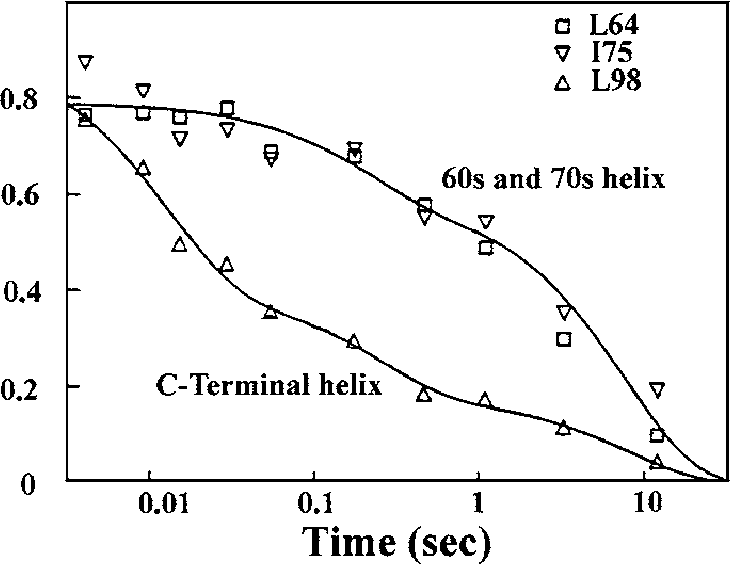
\includegraphics[width=7.0cm]{Figures/CytC.png}
 
 \tiny Englander
 
\end{frame}

\begin{frame}{What can you do with a Markov State Model?}{Ligand Binding}

\includegraphics[width=7.0cm]{Figures/gianni.png}

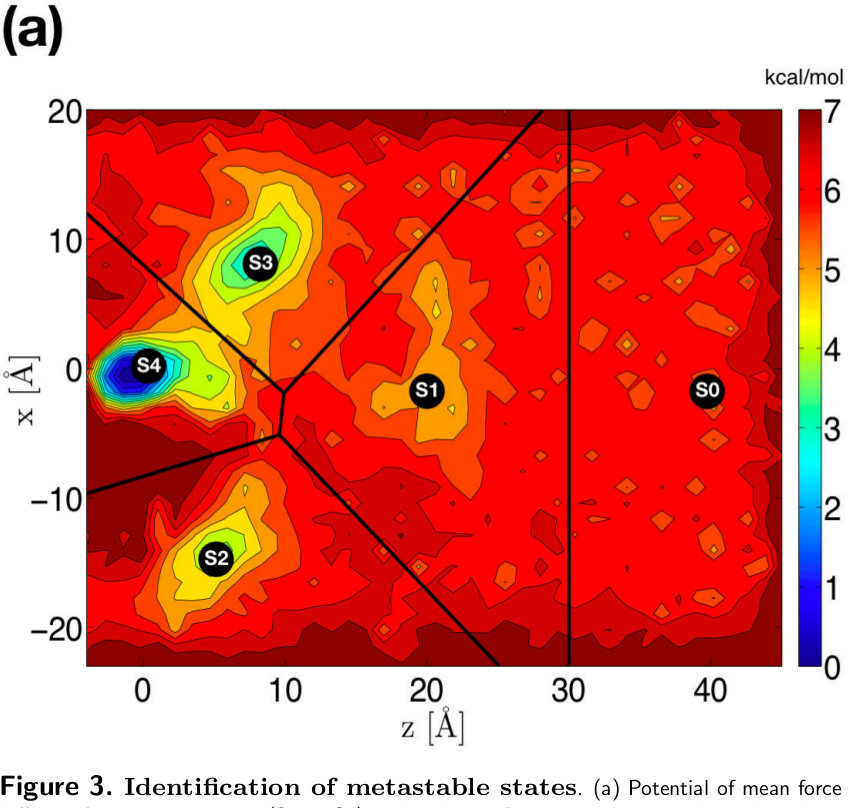
\includegraphics[width=7.0cm]{Figures/gianni_fig.png}
 
 
\end{frame}

\begin{frame}{What can you do with a Markov State Model?}{Predict Experiments}
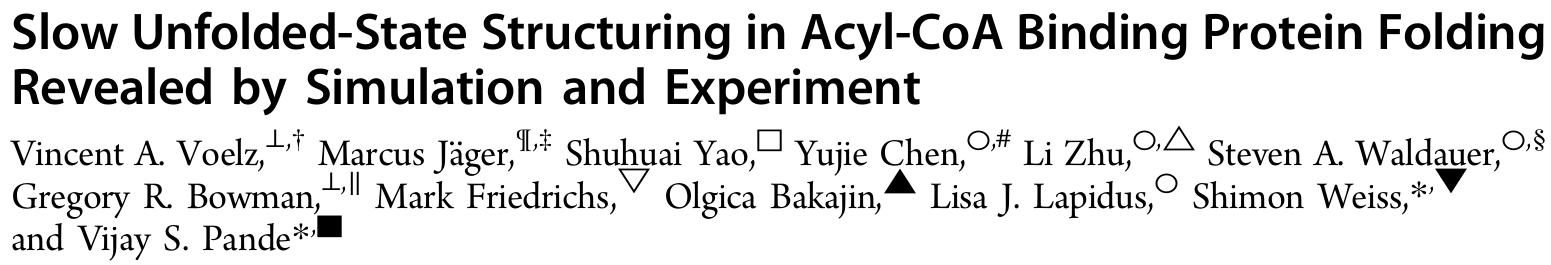
\includegraphics[width=7.0cm]{Figures/voelz.png}

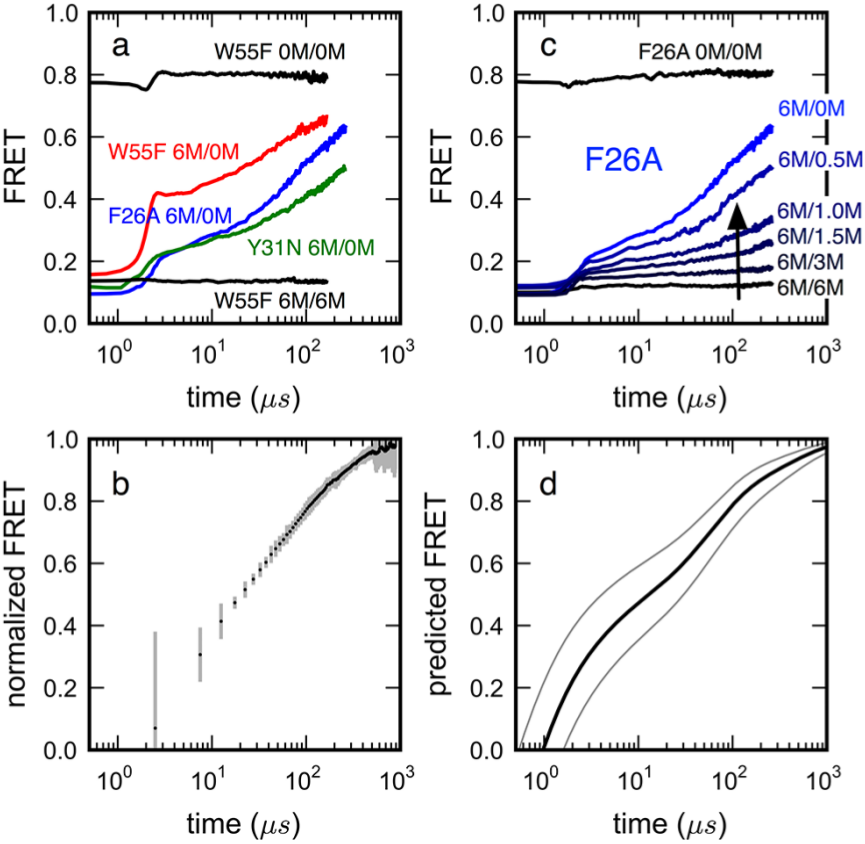
\includegraphics[width=7.0cm]{Figures/voelz_fig.png}
 
 
\end{frame}

\begin{frame}{What can you do with a Markov State Model?}{Construct Simple Models}
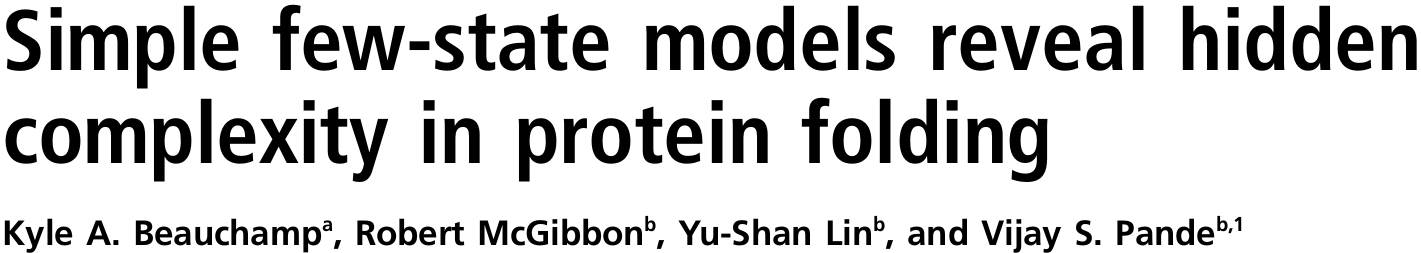
\includegraphics[width=4.5cm]{Figures/beauchamp.png}

\includegraphics[width=9.3cm]{Figures/beauchamp_fig.pdf}
 
 
\end{frame}

\begin{frame}{What can you do with a Markov State Model?}{Extract Pathways}
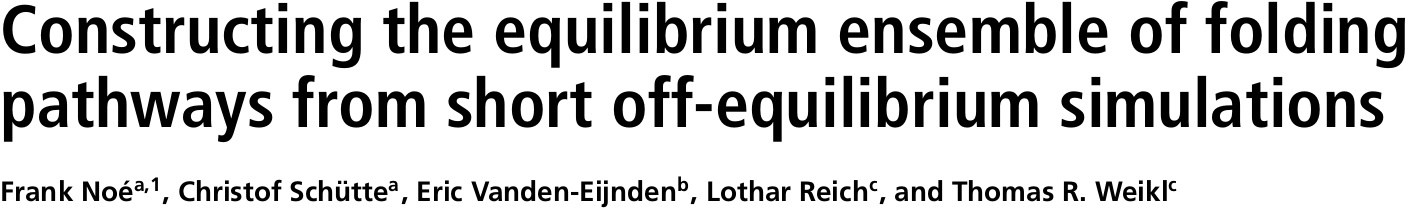
\includegraphics[width=7.0cm]{Figures/noe.png}

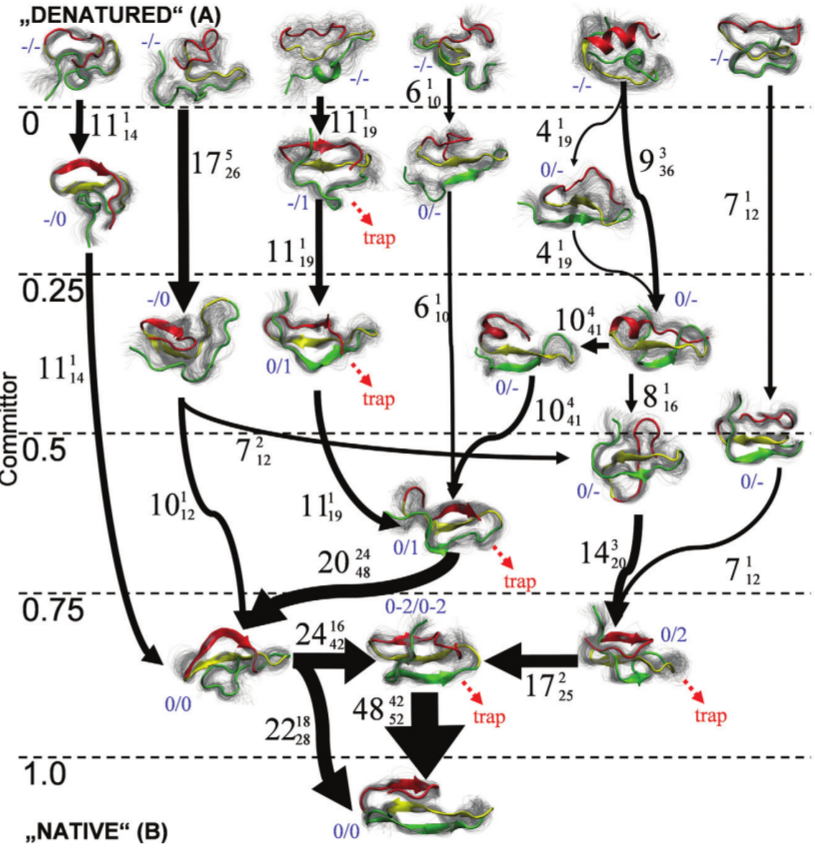
\includegraphics[width=7.0cm]{Figures/noe_fig}
 
 
\end{frame}

\begin{frame}{Introduction to MSMBuilder}{Typical MSMBuilder Workflow}

\begin{columns}
 
 \column{7cm}
 
\begin{enumerate}
 \item Data preparation
 \item Build microstate model (clustering)
 \item Build macrostate model using lumping
 \item Investigate macrostates
\end{enumerate}

\column{5cm}

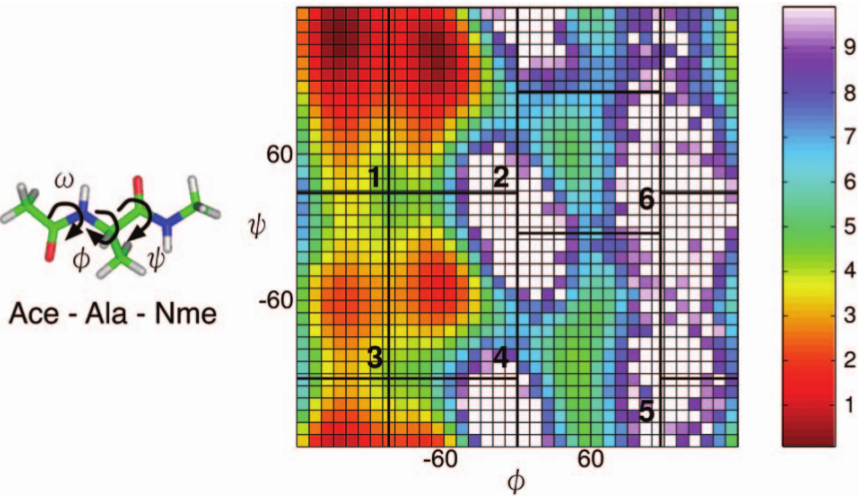
\includegraphics[width=5.0cm]{Figures/chodera}

\end{columns}

\end{frame}

\begin{frame}[fragile]{Data Preparation}
 
Convert XTC trajectories into MSMBuilder (HDF: .lh5) files:


\vfill

\begin{verbatim}
cd ~/msmbuilder/Tutorial
ConvertDataToHDF.py  -s native.pdb -i XTC
\end{verbatim}

\vfill

MSMBuilder can read XTC, PDB, DCD, and other formats.   
 
\end{frame}

\begin{frame}[fragile]{Cluster your data}

To define microstates, clusters your data using the RMSD metric with hybrid k-centers k-medoids clustering.

\begin{verbatim}
 
Cluster.py rmsd hybrid -d 0.045 -l 50
 
\end{verbatim}

\begin{enumerate}
 \item Use the ``rmsd'' distance metric
 \item Use the hybrid k-centers k-medoids clustering algorithm
 \item Stop clustering when cluster radii are less than 0.045 nm
 \item Refine clusters with 50 iterations of hybrid k-medoids
\end{enumerate}
 
\end{frame}

\begin{frame}{How to get help}

Access help at command line with ``-h'' option.


Some help menus are context dependent:

\begin{itemize}
 \item Cluster.py -h
 \item Cluster.py rmsd -h
 \item Cluster.py rmsd hybrid -h
\end{itemize}


\end{frame}



\begin{frame}[fragile]{Clustering Output Files}

By default, Cluster.py will produce three files:

\vfill
 Data/Assignments.h5 is the set of state assignments.
\vfill 
 Data/Assignments.h5.distances is the set of distances from each frame to its assigned cluster.
 \vfill
 Data/Gens.lh5 is the set of cluster centers.
 
\end{frame}


\begin{frame}{Choosing a lagtime}{What is a lagtime?}
 
MSM calculations require the user to pick a fixed lagtime.

\vfill

Lagtime = the time window used when counting transitions.

\vfill

The lagtime can any integer multiple of the trajectory output frequency.

\end{frame}

\begin{frame}{Implied Timescales}
 
 The eigenvalues of the transition matrix provide the ``implied timescales'' of the model:
 
 \vfill
 
 Implied timescales serve three roles:
 
\begin{enumerate}
 \item Choose the number of macrostates via the ``spectral gap''
 \item Choose the macrostate lagtime via ``leveling-off''
 \item Experimental observables decay via a sum of exponentials with these timescales.
\end{enumerate}

\end{frame}


\begin{frame}[fragile]{Calculating Implied Timescales}

\begin{verbatim}

CalculateImpliedTimescales.py -l 1,25 -i 1 -o \
Data/ImpliedTimescales.dat

PlotImpliedTimescales.py -d 1. -i Data/ImpliedTimescales.dat


\end{verbatim}

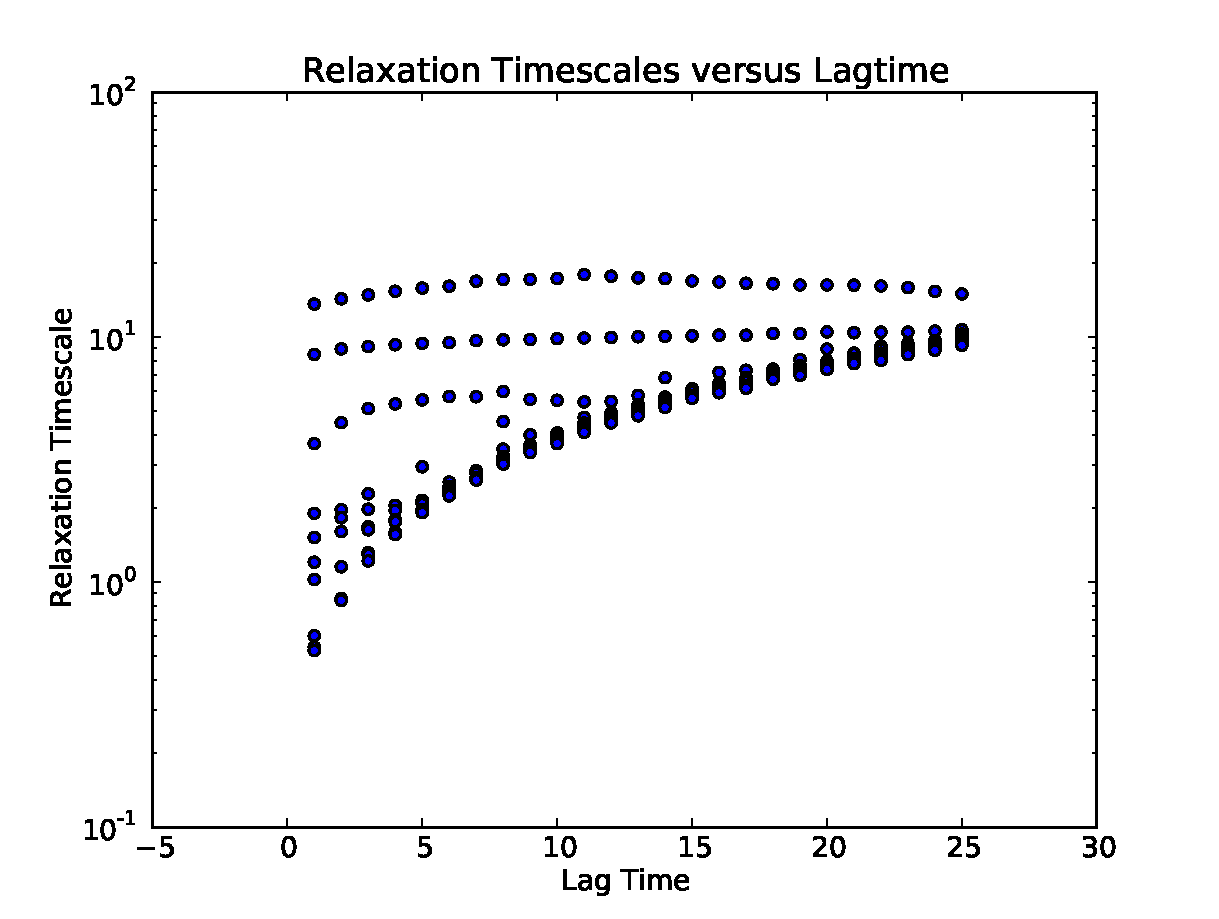
\includegraphics[width=7.0cm]{Figures/microstate_timescales.pdf}

\end{frame}

\begin{frame}{Determine the number of macrostates}
  
 The top 3 timescales are separated by a spectral gap.
 
 \vfill
 
 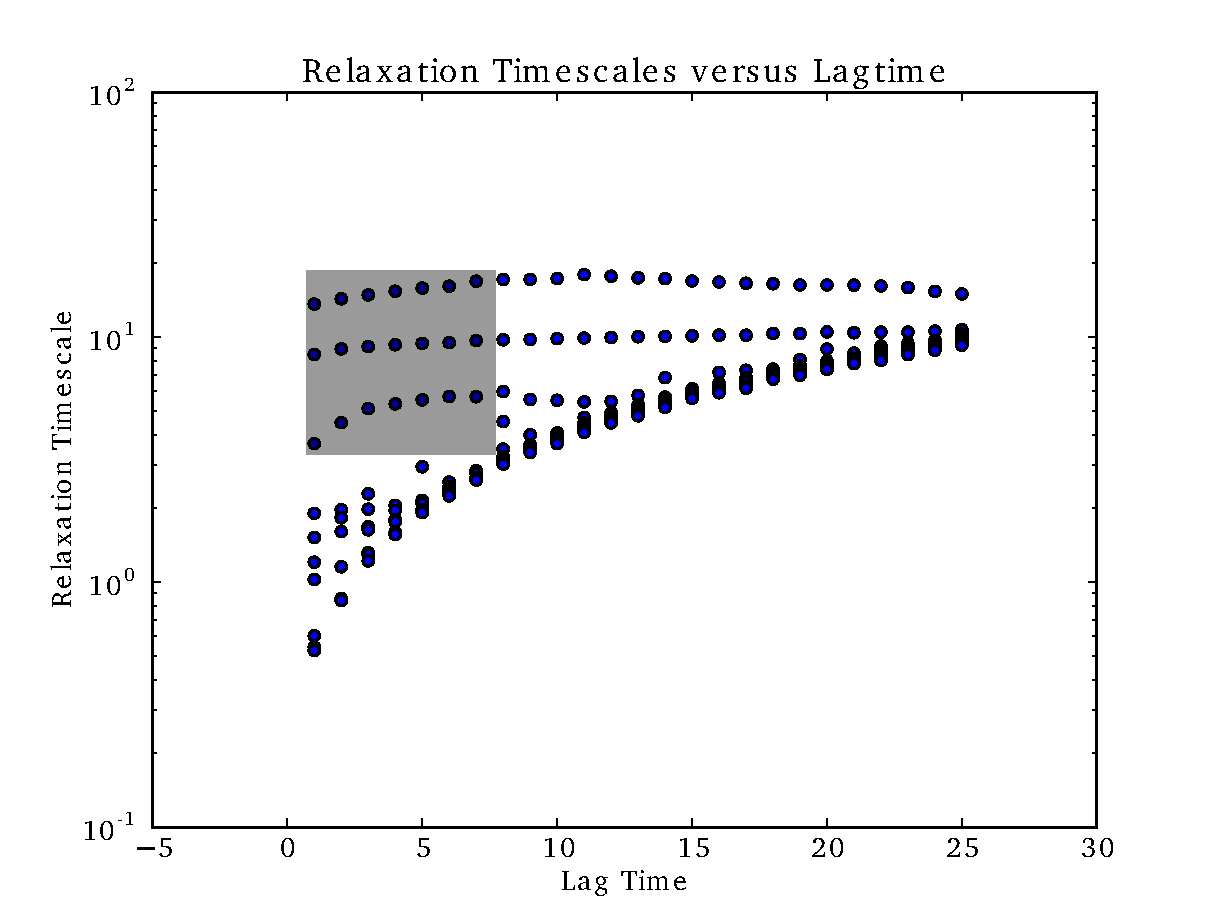
\includegraphics[width=7.0cm]{Figures/microstate_timescales-gap.pdf}

 \vfill
 
 Three slow timescales suggests building a four macrostate model.
 
\end{frame}



\begin{frame}[fragile]{Build a Macrostate Model}

\begin{enumerate}
 \item Build a transition matrix with lagtime of 1 ps
 \item Use the transition matrix as input to PCCA+ algorithm
\end{enumerate}

\vfill

 \begin{verbatim}
BuildMSM.py -l 1 -o L1

PCCA.py -n 4 -a L1/Assignments.Fixed.h5 -t L1/tProb.mtx \
-o Macro4/ -A PCCA+
 \end{verbatim}

 
\end{frame}


\begin{frame}[fragile]{Visualize Macrostates}
 
 \begin{verbatim}
python PlotDihedrals.py Macro4/MacroAssignments.h5
 \end{verbatim}

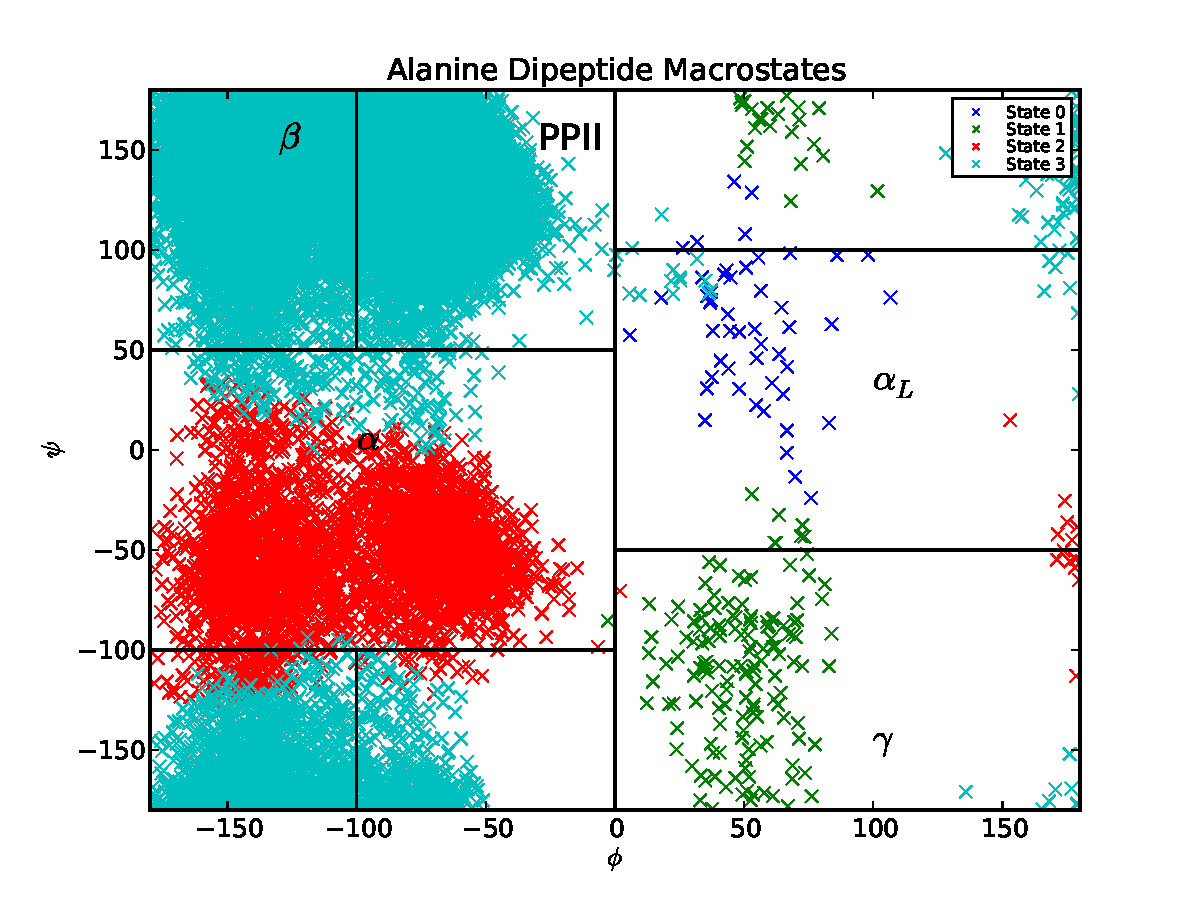
\includegraphics[width=7.0cm]{Figures/Macro4.pdf}

Note the agreement with a manual state decomposition from Tobin Sosnick.
 
\end{frame}

\begin{frame}{Errors in Markov State Models}
 
MSM modeling requires that the data be Markovian, or memoryless.

\vfill

We can use implied timescales to check that data is truly Markovian:


$$\tau = -\frac{\Delta t}{\log(\lambda)}$$


This \emph{implied timescale} should be independent of the lagtime $(\Delta t)$ used to slice your trajectories!
 
\end{frame}

\begin{frame}[fragile]{Validate Macrostate MSM}
 \begin{verbatim}
  CalculateImpliedTimescales.py -l 1,25 -i 1 \
-o Macro4/ImpliedTimescales.dat \
-a Macro4/MacroAssignments.h5 -e 3

PlotImpliedTimescales.py -i Macro4/ImpliedTimescales.dat -d 1

 \end{verbatim}

 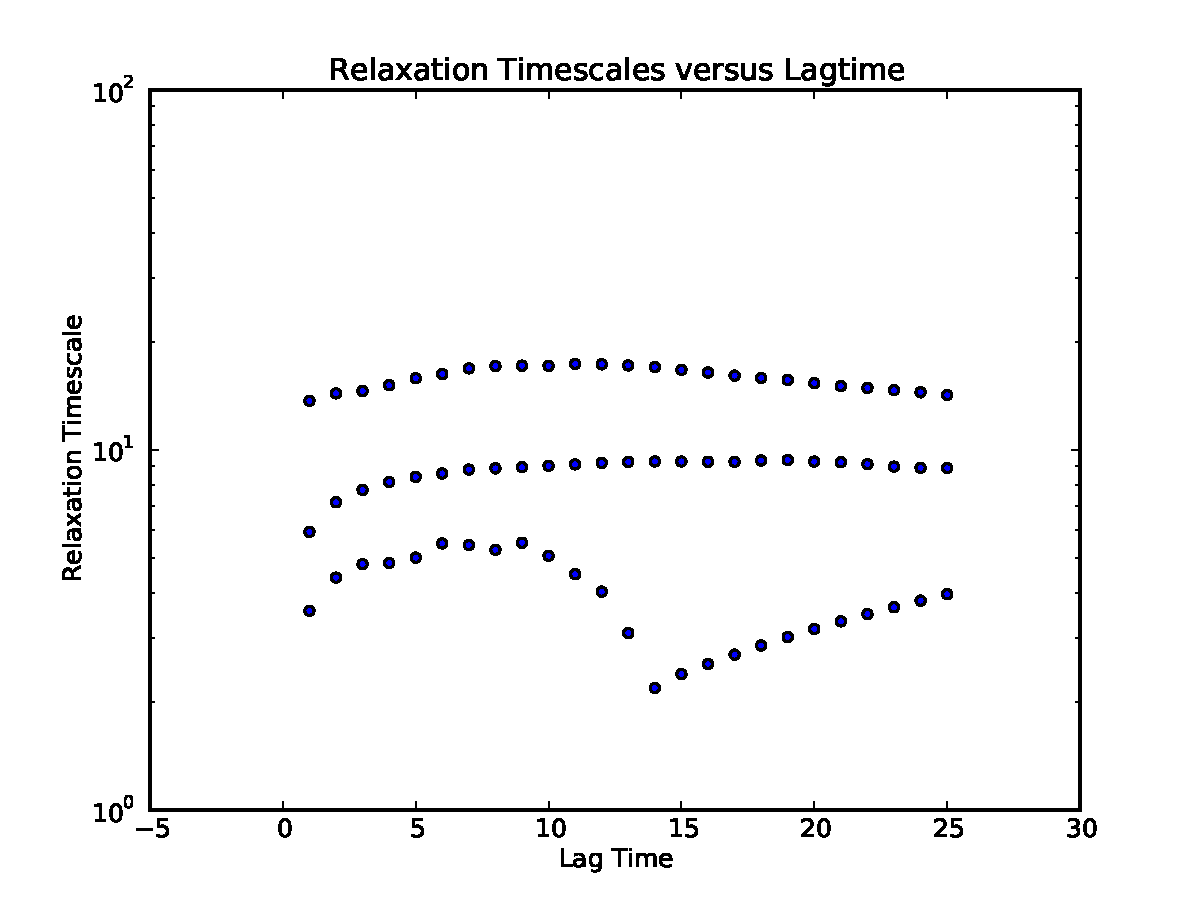
\includegraphics[width=7.0cm]{Figures/macro_implied.pdf}
 
\end{frame}

\begin{frame}[fragile]{Build a ``converged'' model}

Note the convergence at 6 ps.

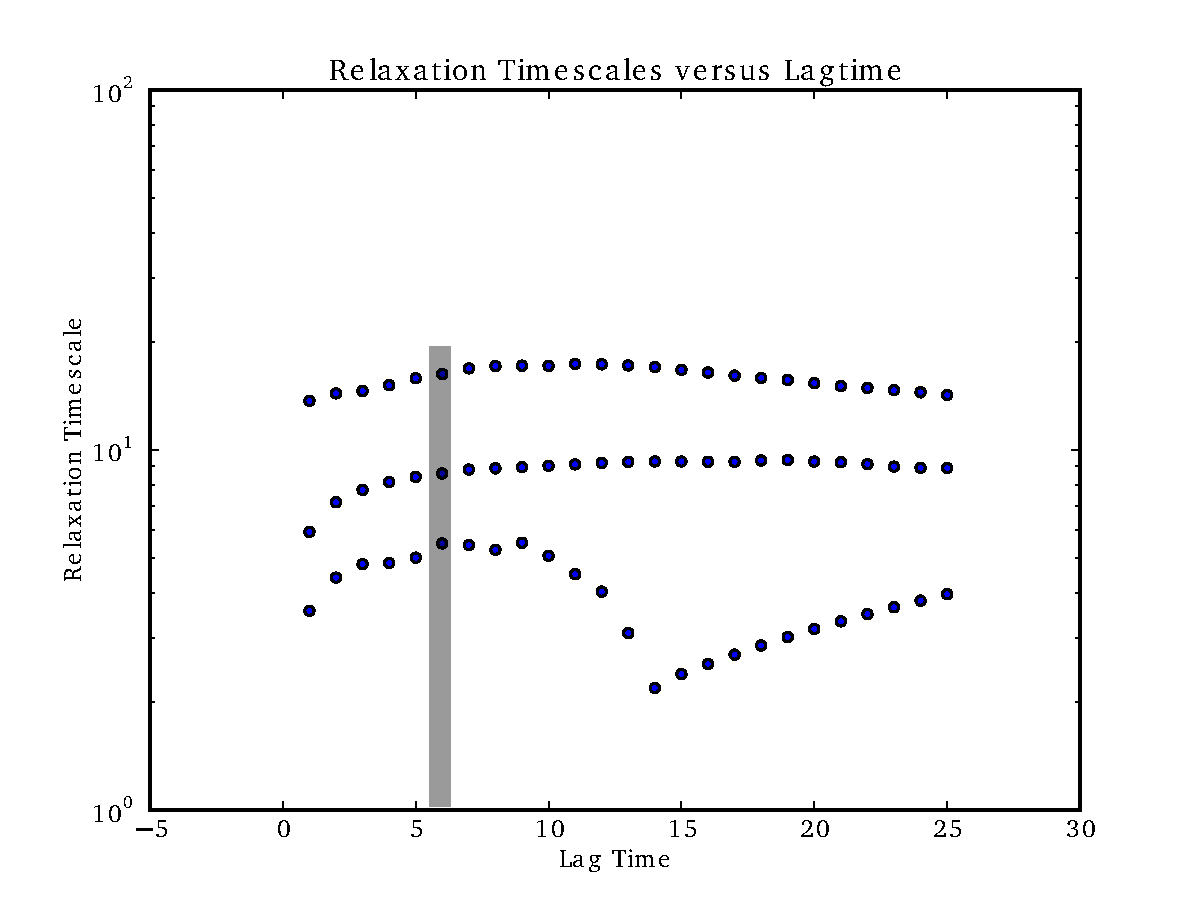
\includegraphics[width=7.0cm]{Figures/macro_implied-cut.pdf}

 \begin{verbatim}
BuildMSM.py -l 6 -a Macro4/MacroAssignments.h5 -o Macro4/   
 \end{verbatim}


\end{frame}


\begin{frame}[fragile]{Save PDBs}
 
\begin{verbatim}
SaveStructures.py -s -1 -a Macro4/MacroAssignments.h5 \
-c 1 -S sep
pymol PDBs/State0-0.pdb PDBs/State1-0.pdb PDBs/State2-0.pdb \
PDBs/State3-0.pdb
\end{verbatim}

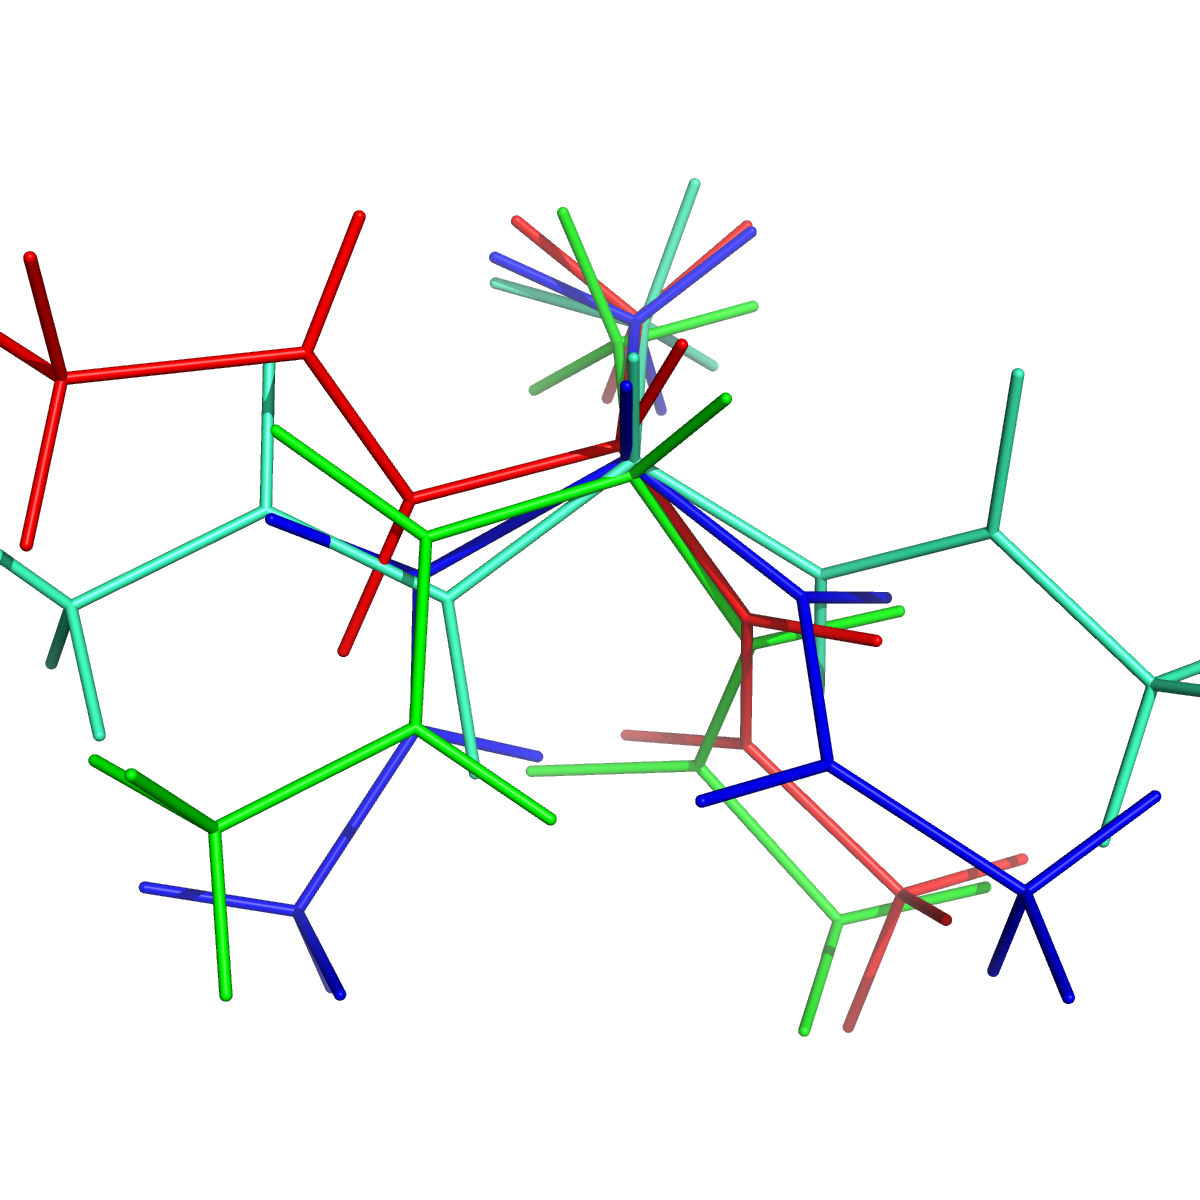
\includegraphics[width=7.0cm]{Figures/ala.png}
 
\end{frame}

\begin{frame}{Visit our GitHub page to report any issues!}{https://github.com/SimTk/msmbuilder/}
 
 
 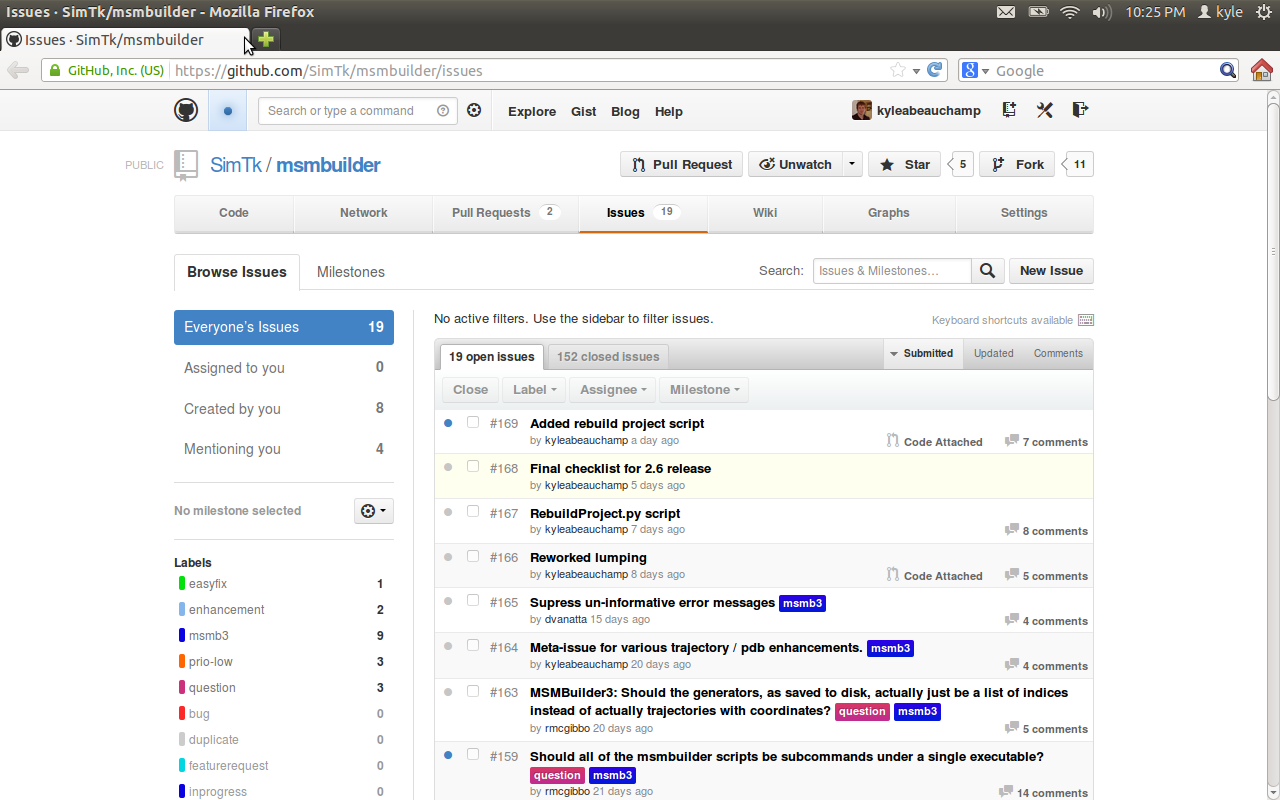
\includegraphics[width=11.0cm]{Figures/GitHub.png}
 
\end{frame}


\end{document}